\subsection{Quadrant III. (Explicit Assurances, Informal Trust Treatment)}\label{sec:q3}
    An AIA that has the capability of predicting its own performance on different tasks can use that to communicate with humans about competence, predictability, and the situational normality of a given task. Several authors have worked to improve this ability in visual classification \cite{Zhang2014-he,Gurau2016-hs,Churchill2015-ei,Kaipa2015-hy}. Some examples from that literature include \citet{Zhang2014-he} who approach the problem by, in essence, learning a model of the training error associated with different images and then using this to predict the error on test images. This ensures that the classifier won't fail silently (i.e. without warning). Also, learning from input data makes their method applicable to any classifier. Also, \citet{Kaipa2015-hy} approaches the problem more from the perspective of estimating the likelihood of a sensed part matching the desired one; this within the scenario of a robot picking parts from a bin. To accomplish this they apply the `Iterative Closest Point' (ICP) method, to match a point cloud measurement of the part with a ground-truth 3d model of the part. Each of these approaches enables the AIA to quantify its capability, and do then present appropriate assurances to the human user.

    It is also important to consider the intrinsic limitations of the AIA in predicting performance. To this end \citet{Kuter2015-qh} propose that an AIA be able to calculate the stability of its planner. In essence they ask: how sensitive is the plan to uncertainties? They use `counter planning' and `plan repair' to enable the autonomous system to identify likely contingencies that might interfere with an existing plan and then adapt the plan to account for those contingencies. Similarly, \citet{Hutchins2015-if} investigate the inherent `competency boundaries' of an autonomous systems' components (i.e. sensors, actuators, planners). The competency of each component can change in different situations such as sunny/stormy weather, or physical surroundings (i.e. variation of GPS accuracy). If these competency boundaries could be quantified (currently by an expert using a Likert scale) then performance in different situations could be more accurately understood (further, they consider \emph{how} this information might be communicated to a user).

    A well-known concept in machine learning and pattern recognition is the trade-off between accuracy and interpretability, or that generally improving the accuracy of a certain model reduces the interpretability. \citet{Ruping2006-xj} specifically asks how classification results can be made more interpretable to those who design and use classifiers. To address the accuracy-interpretability trade-off he investigates the use of a simpler global model, and a more complex local model (\citet{Otte2013-oo} and \citet{Ribeiro2016-uc} implement similar ideas as well). Figure \ref{fig:ruping} illustrates this idea on a simple example, the left (global) model can be used as a large scale interpretable model, while the more complex local model (shown on the right) can be used as necessary when more precise understanding is required. While his focus was on classification, the methods could also be useful in regression as well.

    \begin{figure}[htbp]
    \centering
    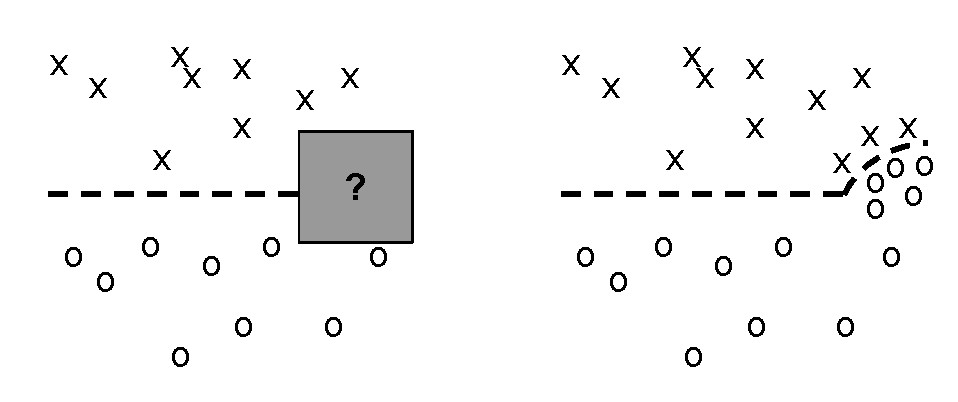
\includegraphics[width=0.8\textwidth]{Figures/global_local}
    \caption{Example of simple global model on the left, and on the right a more complex local model that can be used for interpretability when more detail is necessary.}
    \label{fig:ruping}
    \end{figure}

    Given a model \citet{Van_Belle2013-ph} suggest that there are three methods that help ascertain the level of interpretability and potential utility of models: 1) Map to domain knowledge, 2) Ensure safe operation across the full operational range of model inputs, and 3) Accurately model non-linear effects (compare to categories proposed by \citet{Lipton2016-ug}). They identify certain strengths and weaknesses of different techniques, and finally conclude that there is no method that is clearly the best in all situations. \citet{Huysmans2011-th} experimented with decision trees, decision tables, propositional if-then rules, and oblique rule sets in order to understand which is the most interpretable method. Through experimentation they found decision trees and tables to be more interpretable, but note that each method has applications in which it can perform better than other methods.
    
    While the work of \citeauthor{Huysmans2011-th} gives some indication about how to choose classifiers for interpretability, \citeauthor{Park2016-ld}, who investigated and proposed methods for making interpretable rules in decision trees, points out that to gain \emph{real} interpretability in complex tasks expert knowledge is still needed to make sense of complicated features. As two examples \citet{Jovanovic2016-gw} use `Tree-Lasso' logistic regression with domain knowledge. Specifically they use medical diagnostic codes to group similar conditions and then use `Tree-Lasso' regression that uses that information to make a more sparse model. \citet{Zycinski2012-jj} also use domain knowledge to structure a data matrix before feature selection and classification. 
    
    \citet{Faghmous2014-og} argues that interpretable models are necessary in data science when studying scientific phenomena such as environmental effects. They propose using `theory guided data science' (TGDS) that provides theoretical, interpretable, structure to data science problems. As one example of TGDS \citet{Morrison2016-fz} address the situation where an imperfect analytical model is available. They use a chemical kinetics application where the theoretical reaction equations are well known, and then add a `stochastic operator' over the top of the known model to account for uncertainties.
    
    There has been numerous other research efforts towards making models more interpretable. Generally the methods presented compete with (or excede) their state-of-the-art, less interpretable, counterparts. \citet{Abdollahi2016-vn} investigate making collaborative filtering models more interpretable by using a conditional restricted Boltzmann machine (RBM). \citet{Ridgeway1998-lv} use `weight of evidence' (WoE) as a boosting method that is more amenable to interpretation, and show that WoE is on par with AdaBoost. \citet{Choi2016-by} construct a recursive attention neural network to remove recurrence on the hidden state vector, and instead add recurrence on the visits of patients to doctors, as well as on different diagnoses during those visits. In this way the model is able to predict possible diagnoses in time, and a visualization can be that that indicates the critical visits and diagnoses that lead to that prediction.  

    One of the simplest approaches to helping users understand AIAs is to display the raw data being used, and rely on the human's processing power to make conclusions. In most real applications, however, there are too many individual variables for a human to attend to. Beyond that the human may have to be highly trained to interpret the results. In such situations, dimensionality reduction (DR) and visualization are tools that can be used to help make a model or data easier to understand. \citet{Venna2007-yj} discusses dimensionality reduction as a tool for data visualization for ML, and reviews many linear and non-linear projection methods. \citet{Vellido2012-nm} also discusses the importance of DR for making ML models interpretable. As one example, \citet{Kadous1999-rx} applied this idea in learning comprehensible descriptions of multivariate time series of Australian sign language by making parameterized event primitives (PEPs), which are commonly occurring patterns in the time series. This resulted in features that were more interpretable to human users.

    In some cases it is desirable to keep a complex, less interpretable, model and then try to explain the results to the user. \citet{Lacave2002-cu} address this from the perspective of explaining Bayesian networks. They are concerned with \emph{how} and \emph{why} a Bayesian network reaches a conclusion. They present three properties of explanation: 1) content (what to explain), 2) communication (how to explain), and 3) adaptation (how to adapt based on who the user is). It is not possible to cover all of the ideas that they present in their paper, but they are key to the idea of designing assurances. Some key points are that they highlight the differences between explaining evidence, the model, or the reasoning. These are three key considerations in making assurances. They also discuss whether an explanation is meant to be a description or for comprehension, as well as whether explanations need to be on a macro or micro scale (as mentioned by \citeauthor{Ruping2006-xj}). They also consider whether explanations should occur by two-way interaction between system and user, by natural language interaction, or by probabilities. Finally, when considering adaptation, they hit on another key point of assurances, which is that in general application not all users will require (or desire) the same kinds of assurances. This paper points out many challenges and considerations in designing assurances, and illustrates that, as with the `No free lunch' theorem, there is no single `best' assurance that will address every possible situation. Other discussion regarding how explanations can be presented is found in \cite{Rouse1986-dz,Wallace2001-fm,Kuhn1997-qc,Lomas2012-ie,Swartout1983-ko}.

    Models and logic are not trustworthy by themselves; they may be flawed to begin with, or when certain assumptions or specifications are violated. Thus, there is also great interest in providing assurances that the models and assumptions underlying different AIA processes are, in fact, sound. \citet{Laskey1991-mf} -- with the intention of helping users of `probability based decision aids' by communicating the validity of the model -- notes that it is infeasible to perform a decision theoretic calculation to decide if revision of the model is necessary. She then presents a class of theoretically justified model revision indicators which are based on the idea of constructing a computationally simple alternate model and then to initiate model revision if the likelihood ratio of alternate model becomes too large (see \citet{Zagorecki2015-qy,Habbema1976-xd} as well).

    \citet{Ghosh2016-dl} present a method, in the framework of a practical self-driving car problem, called Trusted Machine Learning (TML). The main approach of TML is to make ML models fit constraints (be trustable). To do this they utilize tools from formal methods to provide theoretical proof of the functionality of the system. They present `model repair' and `data repair' that they can utilize when the current model doesn't match the data, at which point the model and data can be repaired and control can be replanned in order to conform with the formal method specifications. One challenge that presents itself is how to identify the `trustable' constraints, this returns a lot of responsibility to the designer to foresee all possible failures, which is a strong assumption.

    Another possible way to assure a human user is to use the human in the learning process. \citet{Freitas2006-qo} addressed this point with regards to discovering `interesting' knowledge from data, by comparing two main approaches. Given large datasets (as are typical in many of today's problems), human users require assistance from complex systems in order to find patterns and other `interesting' insights. He mentions `user-driven' methods that involve a user pointing out `interesting' templates, or in another method general impressions in the form of IF-THEN rules. He compares these methods to other `data-driven' methods that have been used, and cites other research that suggests that data-driven approaches are not very effective in practice. This is a cautionary tale that many times engineering methods to assist humans are not as effective as we would like to believe. Although, the `user-driven' approach may not fair any better when compared over many users, as each user will likely have different preferences. \citet{Chang2017-kl} also consider a similar, scaled up, `user-driven' approach called `Revolt' that crowd-sources the labeling of images. It is able to attain high accuracy labeling, while also exploring new or ambiguous classes that can be ignored with traditional approaches.

    Validation and Verification (V\&V) typically refers to using formal methods to guarantee the performance of a system within in some set of specifications. Not all practitioners are conscientious that V\&V provides ways to assure users. A prime example is given by \citet{Raman2013-mz}, who developed a way by which a user can provide natural language specifications to a robot and a `correct-by-construction' controller will be built if the specification is valid. Otherwise, the robot will provide an explanation about which specification(s) cause failure. They study this with the goal of implementing the system on a robot assistant in a hospital. Their method involves parsing natural language input (such as: ``Go to the kitchen''), and converting that to linear temporal logic (LTL) that represents a task specification. This is then used to construct a controller if possible, otherwise the `unrealizable' specifications need to be communicated back to the user. This approach is promising in that it presents a way to communicate that a specification cannot be met, although it does not formally account for effects on user trust or TRBs in formulating explanations. The expression of assurances is also asymmetrically limited to cases where the robot cannot meet the specifications. 

\subsubsection{Summary}
    There are a few main approaches that researchers have used to create explicit assurances:

    \begin{itemize}
        \item Making AIA capabilities more interpretable -- using techniques to simplify models, visualize data, explain reasoning and decision making, or to involve humans directly in the learning process is an attempt to create methods that are well-suited to convey assurances to human users. The output of these methods is the assurance, their interpretable form is well-suited to expressing that assurance.
        \item Predicting AIA performance -- it is critical to predict performance in order for humans to understand how AIAs will behave in possible scenarios. By using methods that can predict performance, designers can give AIAs the capability to explicitly communicate regarding competence, predictability, and situational normality to human users.
        \item Ensuring capability of AIAs -- approaches such as model checking, or formal V\&V allow the AIA to assess whether it is still functioning according to its design; this information is useful in making explicit assurances for human users.
    \end{itemize}

    The underlying hypothesis in this body of research is that the proposed methods \emph{should} affect the user's perception of the `competency', and `predictability' of the AIA, or the `situational normality' of the task being performed. However, none of this has been tested by experimentation that gathers self-reported changes in trust. Similarly, there has been no formalization of how the effects that the proposed assurances have on TRBs might be quantified in different applications. In essence this work is only addressing a small subset of important considerations for designing assurances, or the subset that includes the methods by which to calculate the assurance. The experimental testing of the effects of the proposed assurances on both self-reported trust, and TRBs remains open. Indeed, the research in this quadrant is mainly focused on what AIA engineers and designers \emph{think} needs to be explained, or what assurance they \emph{think} users should have. These ideas definitely have merit, but need to be tested to identify if they are effective, to what extent they are effective, and whether there is a more effective, or more efficient way to achieve similar results.
